\documentclass[10pt,a4paper]{article}
\usepackage[a4paper, total={6in, 9in}]{geometry}
\usepackage[latin1]{inputenc}
\usepackage{amsmath}
\usepackage{amsfonts}
\usepackage{amssymb}
\usepackage{mathtools}
\usepackage{graphicx}
\usepackage{float}
\usepackage[usenames, dvipsnames]{color}
\usepackage{fancyhdr}
\usepackage{enumitem}
\usepackage{listings}
\setlength{\headheight}{15.2pt}
\pagestyle{fancy}
\setlength{\parindent}{0em}
\setlength{\parskip}{10pt}
\setlist[enumerate,1]{label=\alph*)}
\setlist[enumerate,2]{label=(\roman*)}
\definecolor{LGray}{gray}{0.9}
\definecolor{DGray}{gray}{0.4}
\usepackage{inconsolata}
\usepackage[T1]{fontenc}
\lstset{language=Matlab, tabsize=2, breaklines=true, postbreak=\mbox{\textcolor{red}{$\hookrightarrow$}\space}, basicstyle=\linespread{0.7}\ttfamily, commentstyle=\color{DGray}} 
\newcommand*\diff{\mathop{}\!\mathrm{d}}



\begin{document}
\title{ENGSCI760 A3}
\author{Benjamin Yi}
\rhead{Benjamin Yi - byi649 - 925302651}
\lhead{ENGSCI760 A3}
	
\section*{Question 1}
\begin{equation*}
f(s) = 5*\bigg| \frac{\sum^n_{i=1} w(s_i)y_i}{\sum^n_{i=1}w_i} \bigg| + \bigg| \frac{\sum^n_{i=1} w(s_i)x_i}{\sum^n_{i=1}w_i} \bigg|
\end{equation*}

\section*{Question 2}
\begin{align*}
t(s, a, b) &= (s_1, s_2, \dots , s_{a-1}, s_b, s_{a+1}, \dots, s_{b-1}, s_a, s_{b+1}, \dots, s_{120}) && \text{if } b > a \\
 &= (s_1, s_2, \dots , s_{b-1}, s_a, s_{b+1}, \dots, s_{a-1}, s_b, s_{a+1}, \dots, s_{120}) && \text{if } a > b \\
&= s && \text{if } a = b
\end{align*}

\section*{Question 3}
We move the container in position \textit{a} to the empty location \textit{b}, leaving position \textit{a} empty.

\section*{Question 4}
\begin{align*}
b = a + 60\longrightarrow &t(s, a, a + 60) && \text{Swapping containers vertically does not change anything} \\
a = b + 60\longrightarrow &t(s, b + 60, b) && \text{Swapping containers vertically does not change anything} \\
w(s_a) = w(s_b) & && \text{Swapping a container with an identical container does nothing}
\end{align*}
Note that as we assume uniquely weighted containers, the third scenario reduces down to \(s_a = s_b\) i.e. swapping a container with itself, or swapping empty containers.

\section*{Question 5}
\begin{equation*}
N(s) = \bigg\{t(s,a,b) \text{ for } a=1,2,\dots,119; \, b=a+1,a+2,\dots,120; \, b \neq a+60; \, w(s_a) \neq w(s_b)\bigg\}
\end{equation*}

\section*{Question 6}
We store extra intermediate variables which correspond to the centre of masses:
\begin{align*}
\text{zy}(s) &= \sum^n_{i=1} w(s_i)y_i\\
\text{zx}(s) &= \sum^n_{i=1} w(s_i)x_i\\
\end{align*}
To update these on each evaluation:
\begin{align*}
\text{zy}(s_\text{new}) &= \text{zy}(s_\text{old}) - w(s_{\text{old}, a})y_a + w(s_{\text{old}, b})y_a - w(s_{\text{old}, b})y_b + w(s_{\text{old}, a})y_b \\
\text{zx}(s_\text{new}) &= \text{zx}(s_\text{old}) - w(s_{\text{old}, a})x_a + w(s_{\text{old}, b})x_a - w(s_{\text{old}, b})x_b + w(s_{\text{old}, a})x_b
\end{align*}
where a, b are equal to the position index swapped for this evaluation. The new objective function is then given by:
\begin{equation*}
f(s) = 5 * \bigg| \frac{\text{zy}(s)}{w_T} \bigg| + \bigg| \frac{\text{zx}(s)}{w_T} \bigg|
\end{equation*}
where \(w_T\) is the sum of the weights of all containers. Note that in implementation, division by \(w_T\) can be left until the end as it is constant and positive.

\section*{Question 7}
Create an array of size n, one element for each container. Initialise the array with some arbitrary value < -h. Whenever a container is swapped, update the corresponding array element to be equal to the iteration count. A container would then be considered banned if (current iteration count - array element value) < h. This requires an array element lookup per container considered each iteration, up to a maximum of 119 * 120 lookups each iteration.

\section*{Question 8}
Instead of recording movement of containers, we could record container positions swapped. This would mean recording a, b instead of s[a], s[b].

\newpage
\section*{Two next-descents code}
\lstinputlisting{A3.py}
\newpage
\begin{figure}[H]
	\centering
	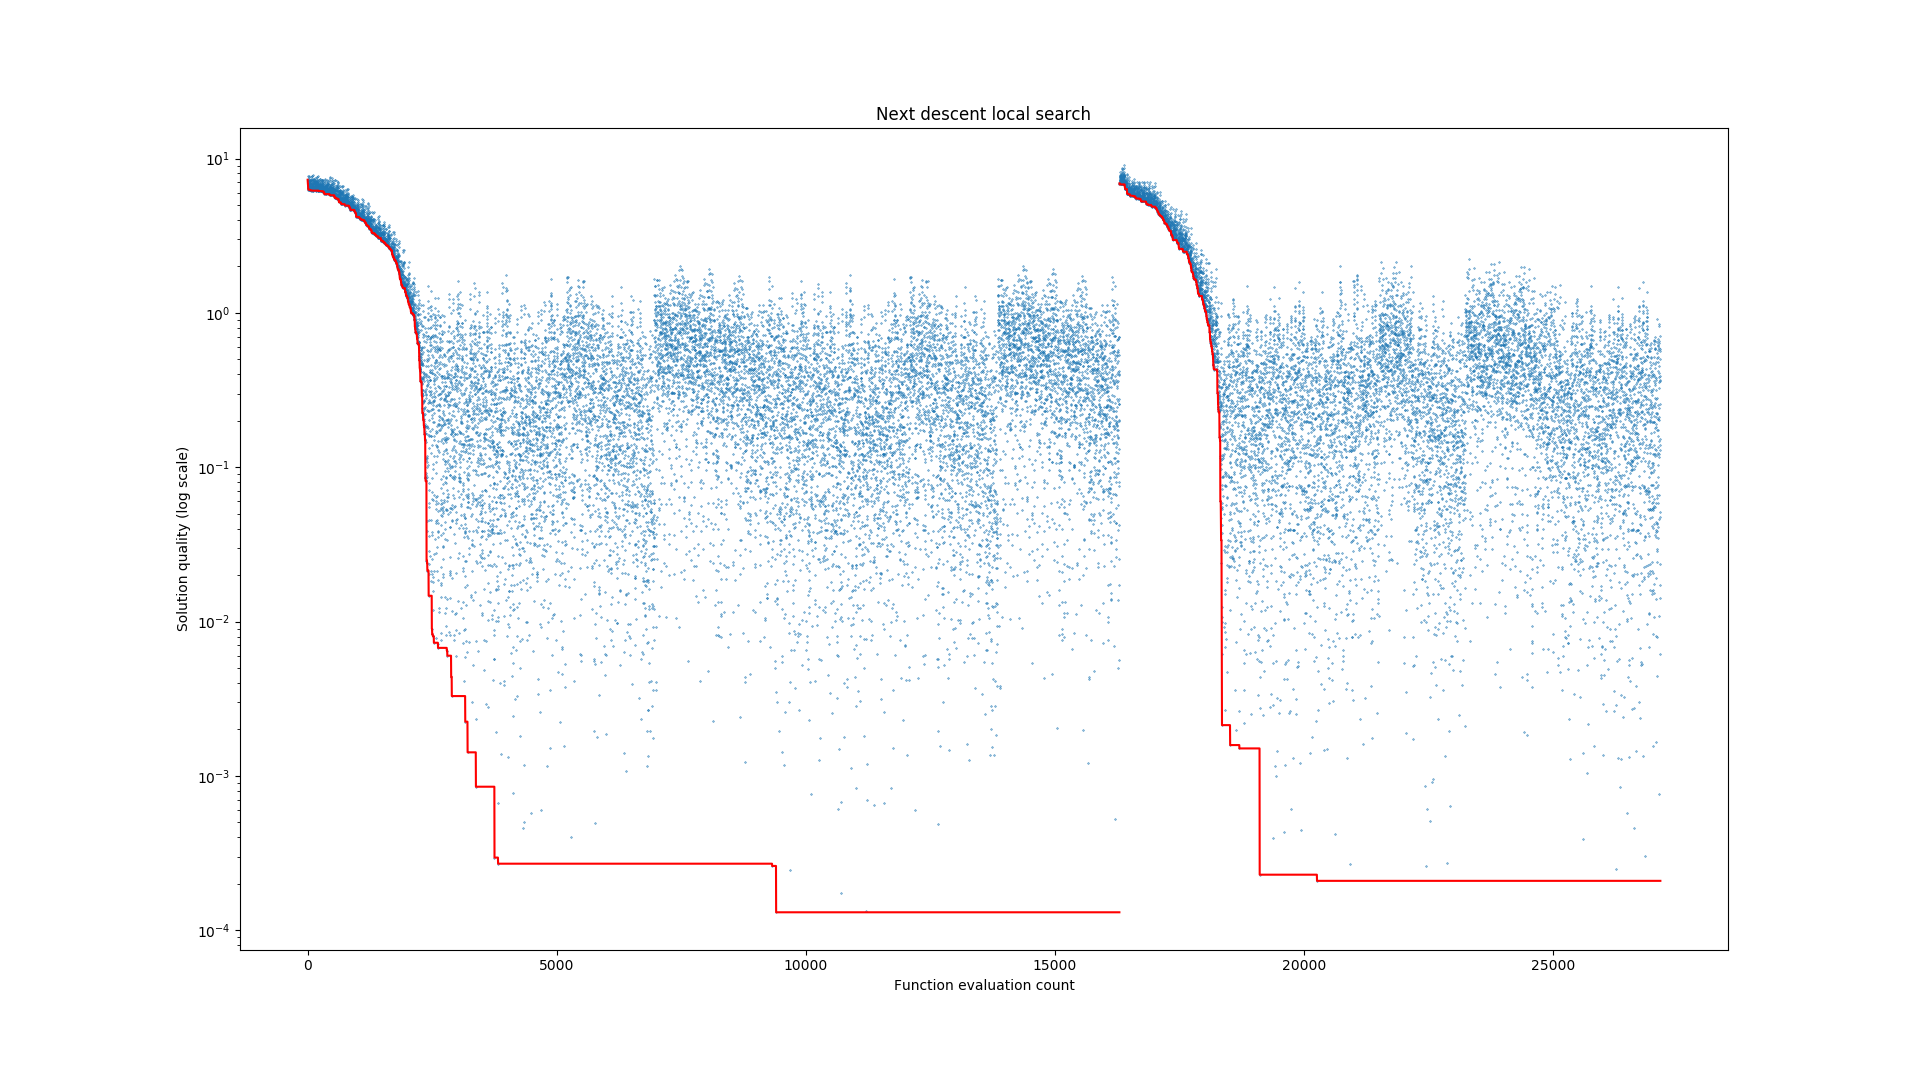
\includegraphics[width=1.8\linewidth, angle=90, origin=c]{2_descent}
\end{figure}


\newpage
\section*{200 iterations code}
\lstinputlisting{200iters.py}

\newpage
\section*{Tabu search code}
\lstinputlisting{tabu.py}
\begin{figure}[H]
	\centering
	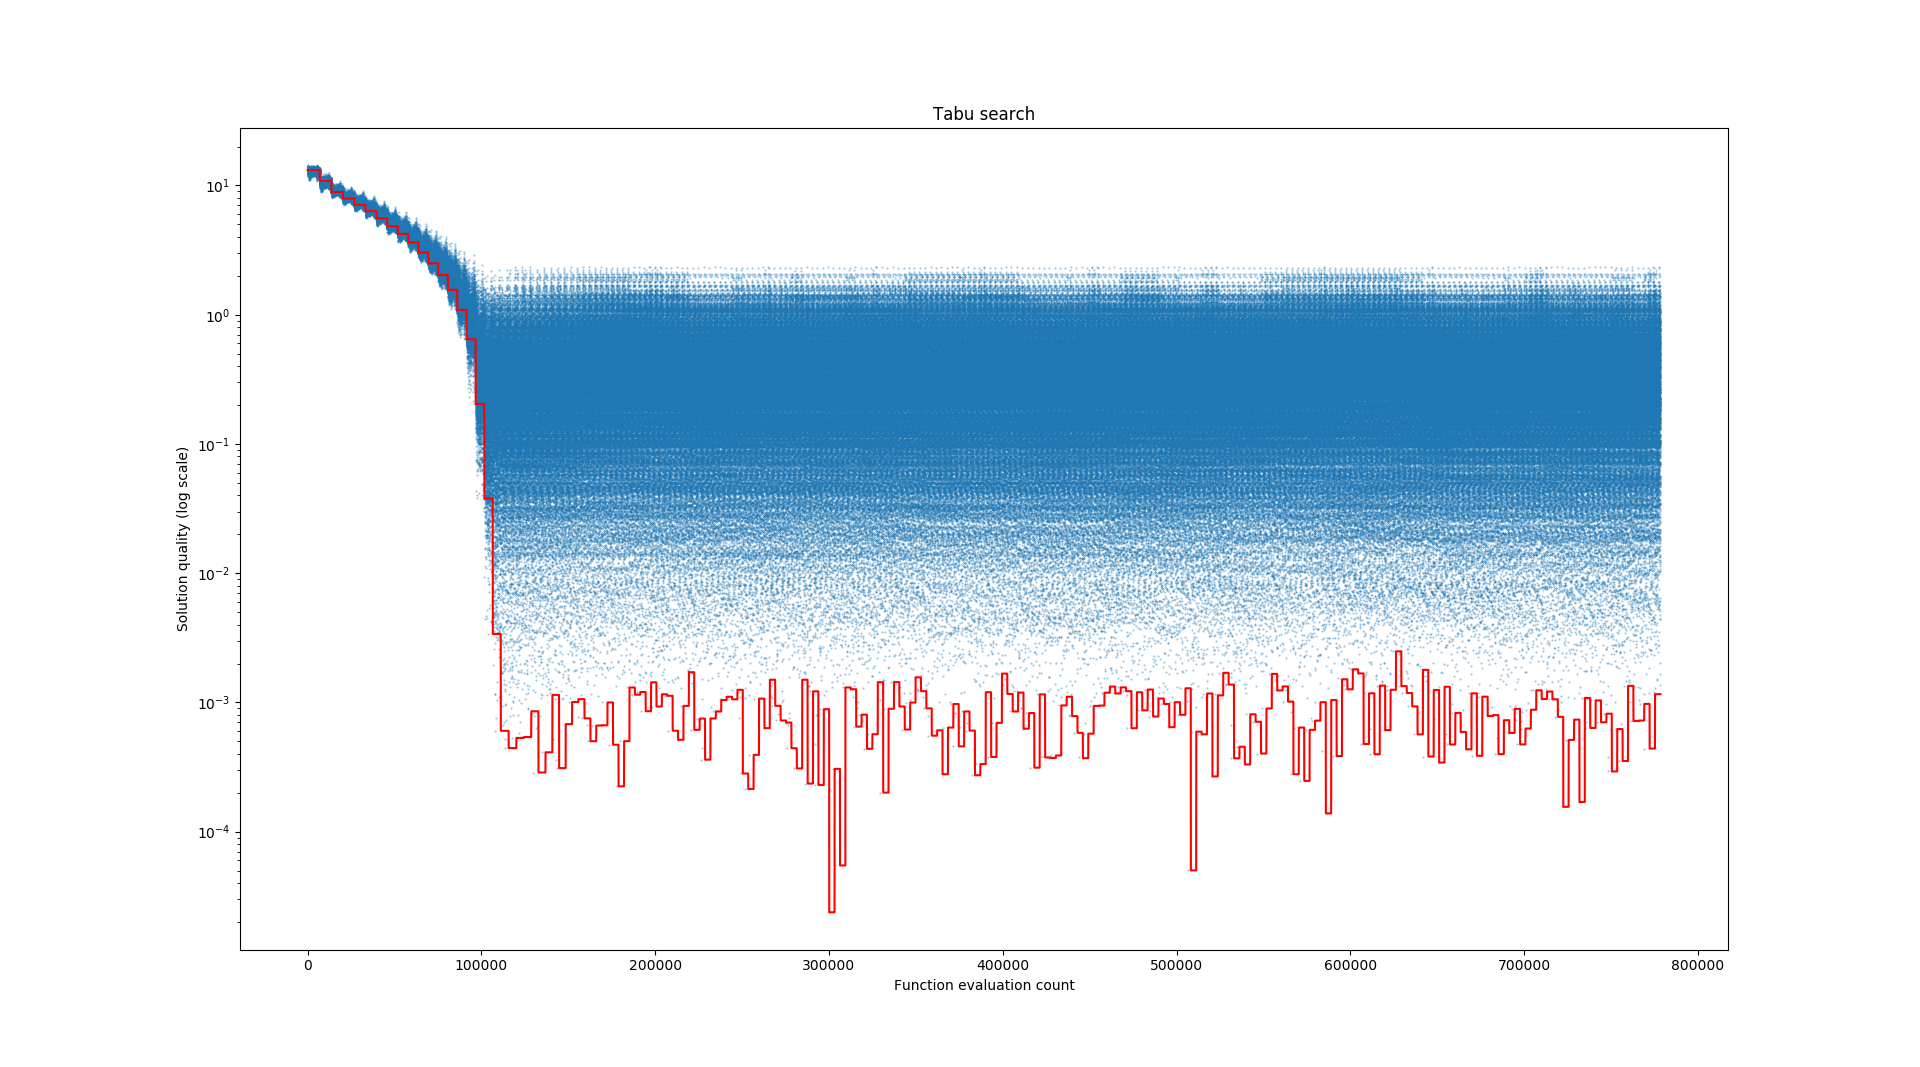
\includegraphics[width=1.8\linewidth, angle=90, origin=c]{tabu_search}
\end{figure}
\end{document}

